\documentclass[10pt,oneside,a4paper]{article}
\usepackage{setspace}
\doublespacing
\usepackage[left=1.5in, right=1in, top=1in, bottom=1in]{geometry}
\usepackage{graphicx} %TO include graphics in document
\usepackage{amssymb}
\usepackage{algorithm}% http://ctan.org/pkg/algorithms
\usepackage{algpseudocode}% http://ctan.org/pkg/algorithmicx
\usepackage{cite}
\usepackage{url}

\author{Arpit Gawande}
\title{DDoS Detection and Defense Using Learning Tool}
\date{\today}
\begin{document}

\begin{abstract}
Distributed Denial of Service (DDoS) attacks are common these days\cite{ddosattacknews}. So it is evident that current industry solutions such as completely relying on Internet Service Provider(ISP) or setting up DDoS defense infrastructure are not sufficient in detecting and mitigating DDoS attacks, hence consistent research is needed. Most of the current industry solutions involve setting up centralized expensive hardware system which can analyze the packets\footnote{Messages that are sent on Internet are broken into shorter messages for transmission. These short messages are called packets. Term coined by Donald Watts Davies.} \cite{networkdatapacket} for probable DDoS attacks. Also each organization or ISP has different systems which are not compatible with other ISP's. In this paper we are going to discuss another a way to detect and mitigate DDoS attack using machine learning tools.
\end{abstract}

\section{Existing Systems}

Distributed Denial of Service (DDoS) attack is the way to jam host network or its resources with large number of data packets, so that host become disabled to serve. There are different types of DDoS attacks such as
1. Volume based e.g. SYN Flood Attacks, in which victim is flooded with hight volume of packets or connection.
2. Application based, in which application such as DNS, VOIP or HTTP where attacked.
3. Low rate DDoS attacks, in which attacker exploit the vulnerability in application design, e.g. Slowloris.
\cite{DDoSAttacks}

The real challenge in detecting and defending DDoS attack is because of its dynamic nature. The source\footnote{It is a system/device on the Internet which has an IP address and which is involved in DDoS attack} is not a single node or system on the Internet but can be many, and often distributed over the Internet. Also the source of the packet is often spoofed\footnote{spoofing is the way to change the source IP address of the message. This is a known issue in the protocol iteself not in the implementation}\cite{ipspoofing}, which makes more harder to know the actual IP address of system from where attack is originated because they hide original attack source. On top of that, many times the source itself is not aware that it is compromised and has been used as bot\cite{bot} by attacker.

Detecting and mitigating attack at the destination\footnote{System under DDoS attack} is not very useful as because destination may know that the attack is happening but to stop it happening it will have to block all the incoming traffic including the legitimate traffic, because source address can not be reliable way to know the attack source. To avoid this, firm which provide the networking devices have come up with solutions.

Many of the solutions available in the market or the research that was done is to collect network traffic flow\cite{networkTrafficFlow} (we would call it just flow) samples at routers(gateways) and feed/send it on the central system to analyze. Central system is a hardware and software infrastructure which is capable of processing and analyzing large flow information.\par

Some of the major protocols which are widely used for flow collection and analysis are, Internet Protocol Flow Information Export (IPFIX) protocol created by Internet Engineering Task Force (IETF), Ciscos NetFlow\cite{cisconetflow} and Sflow(Sampled flow)\cite{sflow}. These protocols have defined standard way to export flow information from router and similar devices. All these flow monitoring protocols gather information and send the consolidated flow information to the centralized server where user can login and do analyses for different purpose such as Security Monitoring, Bandwidth monitoring, Resource Management, Traffic Analysis, Performance Management. It will have some modules which are specifically used for anomaly/DDoS detection.\par

E.g. Cisco netflow has flow Exporter, Collector and Analysis modules. Flow exporter is generally router who send flow information to collector module which acts as flow storage. Analysis module then try to find out different patterns in the flow.\par

These technologies scales well and sufficient to indicate trends in network traffic but they have limitations. 1) They are not cross platform, e.g. router with Sflow protocol would not be able to work with Cisco routers. 2) They involve setting up expensive hardware which would act as collector server. 3) In these technologies source address is used for flow analysis but as we know it is not reliable due to IP spoofing in the case of of DDoS attacks.\par

Now we know that router based flow analysis can be useful for anomaly detection but it has limitations. We don't want to set up expensive hardware, we want to have protocol or system which is compatible with other routers. Also we want to only rely on destination IP address for flow\footnote{Hence forth In our paper we would consider flow only in sense of destination address} analysis. So if we could come up with the way by which we could detect anomaly in the traffic at the routers independent of manufacturer, and create a protocol to communicate the attack parameters to allow routers to take decisions then we would be more efficient in detecting and mitigating DDoS attacks.

If we use the learning algorithm at the router and if router could learn the normal behavior of the flow then if there is any anomaly then it will be able to identify it from its previous learning and that change in behavior of the traffic can be communicate to destination network.

With the advance of electronic and the Internet of things, electronic devices are getting equipped with faster processor and fast memories. Router are also not left behind. Only thing that is missing is the storage space. If we use the learning techniques which don't need much storage then we don't have to store the packets instead we would learn from every flow and discard once learning is done. This is necessary because number of entries on the Internet routing table has steadily grown. Now that the table has passed 500,000 routes\cite{routingtablesize} so storing each and every flow information for these routes could be difficult.\par

\section{DDoS Detection and Mitigation}
One of the way to detect the DDoS attack is to check for anomalous behavior in the network traffic. This can be done at different points. Either at the destination server or at the router. Once the attack is detected by observing the behavior of the traffic to mitigate it, we would have to block all the packets which are causing the attack. One of the way to identify those packets is by their source address.

\section{Network Functioning}
A switch creates a network and router connects networks. A router links computers to the Internet through other routers. Routers are the backbone of the network who helps to forward packet from one point to other point on the Internet. Every packet traveling on Internet has to go through router\cite{swithcrouter}.Router knows where the packet is destine hence it could serve as first point of knowledge about the change in the flow information for a destine network. Each router has interfaces to which hosts or other network are connected. So router is aware to whom it is connected. Router uses protocol to communicate and by that they gather knowledge about other networks or router on the Internet. ICMP\cite{icmp} is one of the most frequently use protocol by routers to communicate.\par

\begin{figure}[H]
\centering
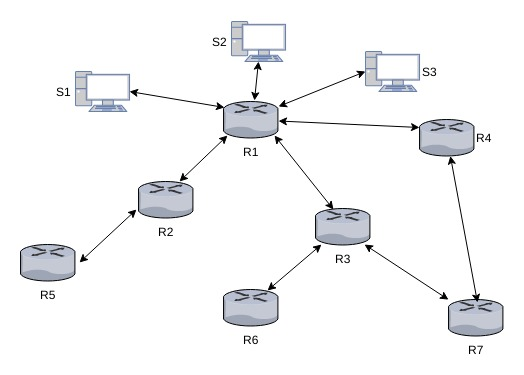
\includegraphics[width=0.80\textwidth]{Routers}
\caption{Network Example} \label{fig:routers}
\end{figure}


Lets illustrated this using an example. In the above figure we can see that host S1, S2, S3 are connected to router R1. Router R1 is connected to Internet through router R2, R3, R4 , thus every packet that would be reaching to S2 would come from either of these three routers. All three routers are locates at different geographical region. Most of the websites are regional, either county, state or national (If we leave out few global websites) and hence they are mostly accessed from those region it is meant for. E.g. Rutgers University website would be accessed mostly from the eastern region of United States and that too mostly from the New Jersey State or the Philadelphia region.\par
Using traceroute we can find out how many hope away the destination is. Each hope is the router on the Internet. Following is one of the captured traceroute for Rutgers University website.\par
%\vspace{5mm} % vertical space
\begin{figure}[H]
\centering
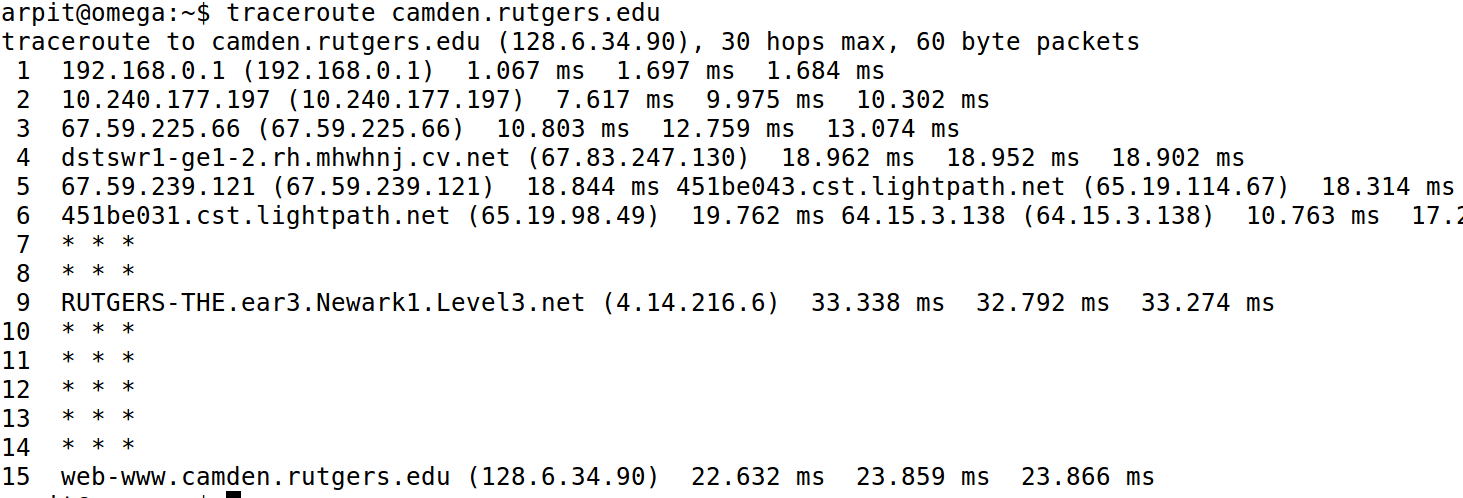
\includegraphics[width=\textwidth]{TraceRoute}
\caption{Trace Route: All the routers in the path to destination} \label{fig:traceroute}
\end{figure}

We can see that there are about 14 routers (if we don't consider the home router 192.168.0.1) to reach to the camden.rutgers.edu. This trace route is taken from a location in the New Jersey State.\par


\section{Suggested New Approach}
From Figure \ref{fig:routers} and \ref{fig:traceroute} we know that routers are located at different geographical locations and also we know that there is pattern in which the particular destination website is getting accessed from the different regions. Some of the service providers such as  GeoIP or Google can find out the location from where the traffic is coming in the network for a given destination, but that is approximate based on the source IP, which in the case of DDoS attack is unreliable information because packet source address are often spoofed. So it could be difficult to know the actual geographical location from which packet has come. Only routers can provide the correct geographical information about the source of the packet.\par

In the normal scenario there would be some definite pattern in which the website is getting accessed from different regions and this pattern can be learned over the time with learning algorithms at the routers. Thus finding this pattern in the flow at the router can form the basis of our analysis. When ever there is deviation from the normal pattern of the flow for a particular destination then that change in pattern as well as the geographical region can be communicated to the destination network. Destination network on receiving that information can decide based on the region and how much is the deviation from the normal to decide whether it want the reporting router to discard or forward the traffic for the destination. This is selective process in which traffic from other routers remain unaffected\par

\begin{figure}[H]
\centering
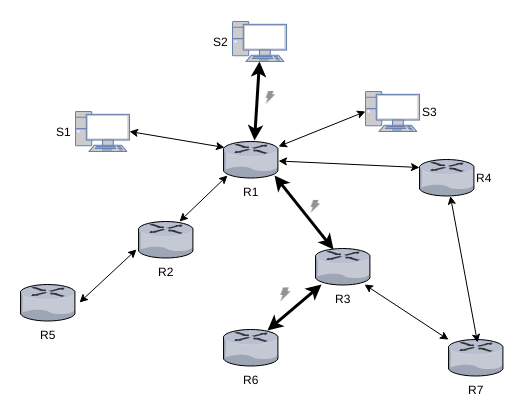
\includegraphics[width=0.90\textwidth]{RouterCommunication}
\caption{DDoS Attack path} \label{fig:attackpath}
\end{figure}


In the above figure attack initiated from the region where router R6 is located and from R6 data packets reach to victim\footnote{Victim is a computer system which is under DDoS attack} from R3 and R1. If we could detect attack at R6 itself then we can discard packets at R6 which are heading towards S2, while traffic from other routers remain unaffected.

To achieve this we would measure the flow during a time window (e.g 300 sec) whose size would be fixed at the beginning.
These time windows can be combined to form a period which is a portion of a day during which traffic is measured. Once we have flow information we can apply learning techniques on each flow iteratively to gain deeper knowledge about normal behavior of the flow.\par

In the proposed system, each router will itself act as a analyzer. Each packet will be analyzed and flow statistic would be created based on the destination IP address. Based on the statistic we would cluster destination IP address using input feature vector. Clustering is the process of examining a collection of “points,” and grouping the points into “clusters” according to some distance measure.The goal is that
points in the same cluster have a small distance from one another, while points in different clusters are at a large distance from one another\cite{machineLearning}.

\begin{figure}[H]
\centering
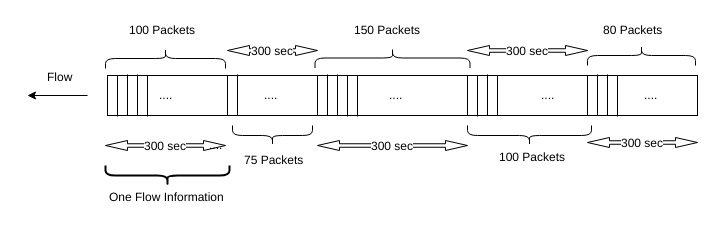
\includegraphics[width=0.90\textwidth]{Data_Flow_Capture}
\caption{Data Flow Segments} \label{fig:flow}
\end{figure}


Once cluster is learned it would be used as bench mark for all future flow. Router would constantly keep clustering destination IP and if there is deviation in the normal traffic at router for a destination then that would affect the clustering and would cause destination to be placed in different cluster, cluster with more packet frequency. This change in clustering would be reported to destination network, which then decide on regulating the traffic\par

\section{Implementation}
There are different types of DDoS attacks such as Volume based, Application based and also Low rate DDoS attacks. Among which the volume based attacks are most common. In the volume base attack victim is flooded with high volume of Internet packets (TCP, UDP, HTTP or ICMP)

We would stick to the volume based attack for the demonstration of our approach and we would try to simulate Bot attack. Bots are the compromised system controlled by attacker for launching attack. They are not bounded by geographical boundaries so can be anywhere in the Internet. Botnet(Network  of bots) are employed by attackers to launch DDoS attack. As we know that Internet is connection of different computer system which can communicate with each other. This communication can occur trough cables, satellite or radio device called communication channels, and these communication channels run through out our world connecting different computer systems at different locations.

We are going to use Wireshark, an open source tool, for capturing Internet packet. Wireshark can capture all digital information received or send through devices such as Ethernet devices, which connects computer to the Internet. It also helps to segregate data in terms of packets pertaining different protocols (e.g. TCP, UDP).\par

\begin{figure}[H]
\centering
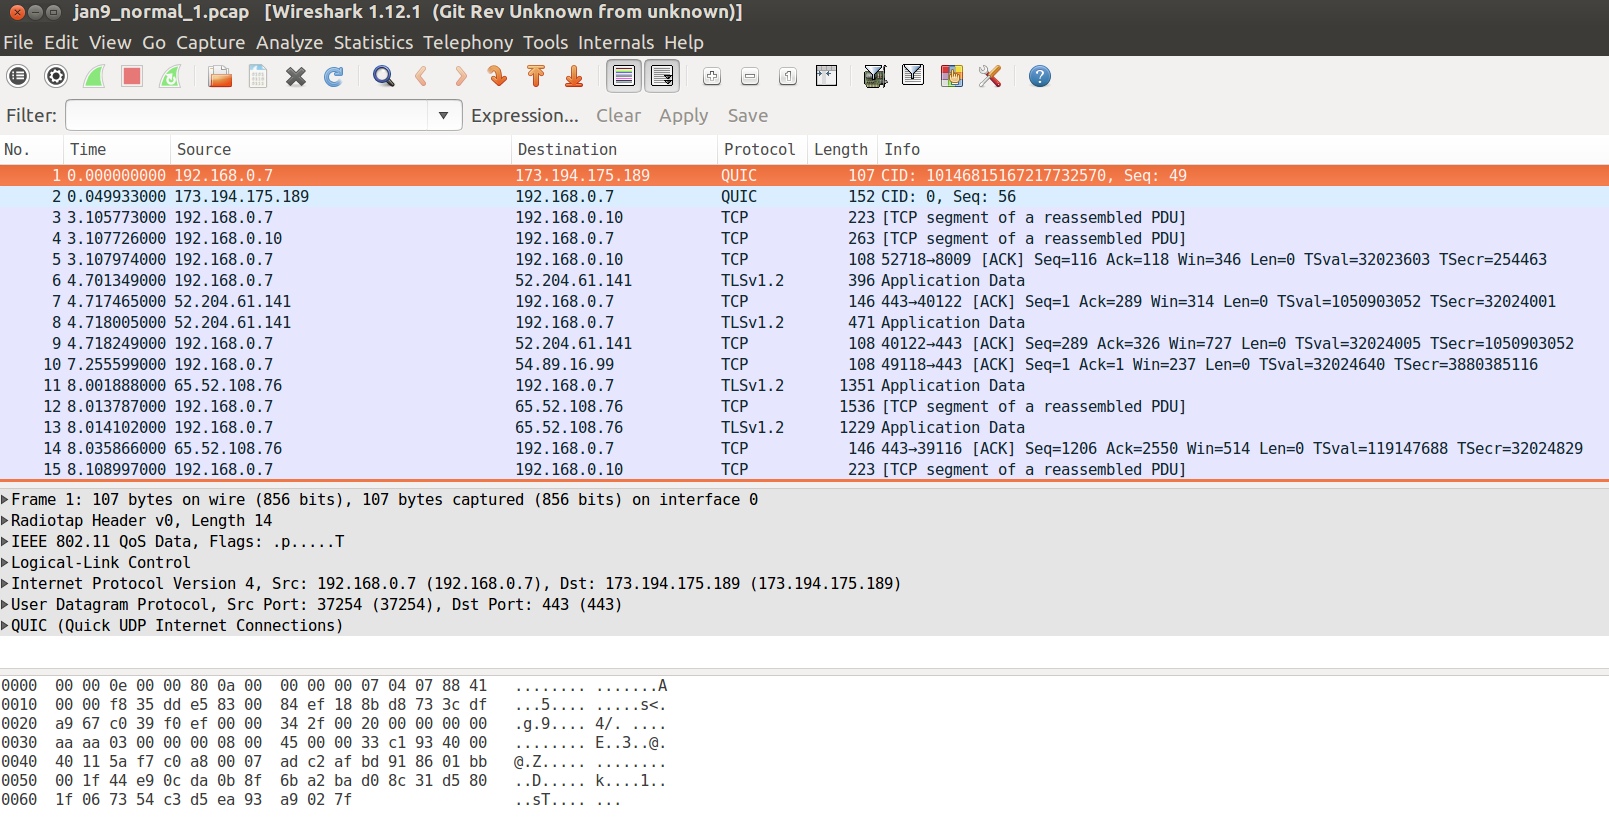
\includegraphics[width=0.90\textwidth]{Wireshark_Tools.png}
\caption{Wireshark Tool: snippet of captured packets} \label{fig:wireshark}
\end{figure}

To gather data for the demonstration we have created a small network with one router and we designated a host machine in that network as a target for the DDoS attack. We have also installed Wireshark on one of the system in the same network. For capturing traffic in the network we are using the Promiscuous mode in Wireshark. Using this mode network interface can record not only the traffic that is intended to its self but all of the traffic on the network. This setup is similar to capturing traffic on a router which is connected to few host machines.

\begin{figure}[H]
\centering
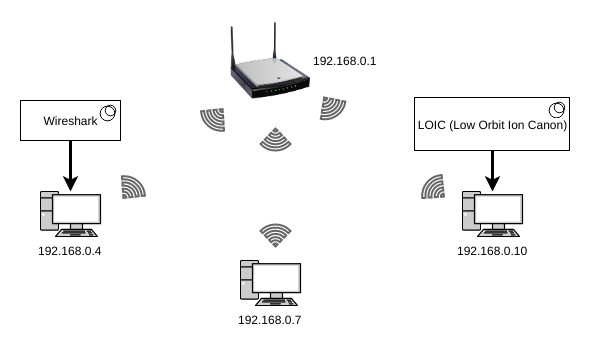
\includegraphics[width=0.90\textwidth]{demo_network}
\caption{Demo Network: for purpose of demonstration} \label{fig:demonetwork}
\end{figure}

Once we start Wireshark we did let it run for a while and then we orchestrate an attack on one of the host (e.g. 192.168.0.4 in Figure \ref{fig:demonetwork}) in the network from another host(e.g. 192.168.0.10 in Figure \ref{fig:demonetwork}) from the same network.

For the sake of simplicity we would be dealing with TCP and UPD flood attacks.

Attack is engineered using Low Orbit Ion Canon(LOIC, a free tool which is even used by attackers in the real world DDoS attacks. This tool allows us to launch TCP and UDP flood attack on any destination. In this paper we would be analyzing the flow based TCP and UDP attack, which is one of the most common type of DDoS attacks.
In the LOIC tool we need to give IP address and the port number of the destination where we want to orchestrate attack while rest of the work is done by it. This tool flood destination with packets and if we choose TCP then it will try to create multiple connections and send packets over them. We start flood attack on one of the system in our network (e.g. 192.168.0.7) and let it continue for few minuets. We launched such attacks few times in between our packet capturing session.

All the traffic including the normal and the attack traffic will get captured in the Wireshark. Packets are captured for about five hours in the given network. Once the packets are captured they are saved as pcapng file which is a Wireshark file format for captured packets. Captured packets during the normal operation and during the attacks are saved separately. The normal packet flow information is used for training and testing the learning algorithms while attack packets flow information would be used for detecting the attack (Which would be explained further in the paper). Wireshark capture every detail of the packets but we don't need all of the information, we would only be interested in the IP layer information of the packet. Most of the routers analyze IP layer of the packet for routing. Having said that there is no reason except than the performance that other layers of the packet are not analyzed.\par

To extract IP layer information from the captured packets data extraction program \textit{data\_extraction} is written in Python. This program would extract address, port and time information from each of the captured IP packets\footnote{packets containing IP information}. It will also divide the captured data into 300 seconds capture window thus creating a sample data which is collection of IP packets captured over the time of 300 seconds. It then write each sample in separate file for further processing. Every sample file represent a one flow information where flow is logically treated as the IP packets captured over 300 second time interval as explained before. This sampling of the packets in the form of flow is the continuous process. Will store the flow information in the form of sample files, we will train learning algorithms using those sample file, then those sample files will be discarded and new samples will be used for further training. This training process has to be continuous process in order to correctly reflect the current status of the flow at given router. What ever the new information is learning is augmented with the previous learning to have the correct understanding of the flow.

This learning can be done for the time during the day or given day during the week of year. e.g. We can have separate learning information for flow from morning 9 am to 12 pm and also can have information for evening 6 pm to 12 pm.

\begin{table}[h!]
\centering
  \begin{tabular}{| l | c | l | c |}
    \hline
    Destination IP      & Protocol  & Time stamp(Sec.)  & Sample Number \\
    \hline
    52.6.129.72         & 6         & 1512094785.928596000  & 1 \\
    192.168.0.4         & 6         & 1512094785.946987000  & 1 \\
    192.168.0.4         & 17        & 1512094786.148488000  & 1 \\
    \hline
  \end{tabular}
\caption{IP packet attributes} \label{table:attribute}
\end{table}

The sample files created using the \textit{data\_extraction} program will be used to create the training set.

Flow based model is build as it is more reliable and fast. Packet analyzing is often difficult due to size and encryption. Also destination port number is not a reliable information in detecting attacks because of the fact that attacker use different ports during attack.

Creating training set is an intermediate step in which IP packet count for each destination for given protocol(e.g TCP, UDP) is calculated. The training set gives us the flow information for each destination (i.e. how many packets are going to given destination IP address during a time window e.g. 300 seconds). We are using \textit{IP\_clustering} Python program to create training set. Our training set look like following in which each row is the destination IP address and columns are the number of packets observed of particular protocol during 300 second time.

\begin{table}[h!]
\centering
  \begin{tabular}{| l |c | c | c | c |}
    \hline
    & \multicolumn{3}{ |c| }{IP Packet count} \\ \cline{2-4}
    {Destination IP}  &ICMP  &TCP &UDP\\
    \hline
    172.217.10.134  & 0     & 8     & 12 \\ \hline
    65.19.96.252    & 5     & 0     & 192 \\ \hline
    68.67.178.134   & 0     & 78    & 0 \\ \hline
  \end{tabular}
\caption{Training Set with three training examples} \label{table:feature}
\end{table}

This training set will be used to train our clustering algorithm. Clustering algorithm separate training examples into different group based on the features, called clusters. We will explain this algorithm in our later section.

There are around 150 protocols managed and assigned by Internet Assigned Numbers Authority (IANA) but most commonly used protocols in the DDoS attack are the ICMP, TCP and UDP protocols. For our training and analysis purpose we are using only these three protocols as the desired feature. In the larger system such as routers managed by ISP, other protocols can also be used as features if required.\par

\subsection{Machine Learning}

According to Tom Mitchell (1998) A computer program is said to learn from experience E with respect to some task T and some performance measure P, if its performance on T, as measured by P, improves with experience.

There are many algorithms which can be used for learning from the data and make the prediction. The learning algorithm build a model/hypothesis using training set as input and that model/hypothesis is used to perform predictions. Most common categorization of machine learning algorithm is Supervised and Unsupervised.

Let $f$ be the function which we need to guessed from input vector X = $x^{1}$, $x^{2}$, ..., $x^{m}$ and $h$ be the hypothesis about the function $f$. $h \in H$ and $f \in H$, where $H$ is class of functions. Both $f$ and $h$ can be vectors. We select $h$ based on a
training set, $\Xi$, of $m$ input vector examples. In Supervised leaning we know the values of $f$ for the $m$ samples in the training set $\Xi$. We assume that if we can find a hypothesis, $h$, that closely agrees with $f$ for the members of $\Xi$, then this hypothesis will be a good guess for $f$ when $\Xi$ is large. In Unsupervised learning, we simply have a training set of vectors without function values for them. The problem in this case, typically, is to partition the training set into subsets, $\Xi_1$,  ,$\Xi_R$, in some appropriate way.\cite{machineLearning}

Supervised algorithm such as One Class Support Vector Machine(One Class SVM)\cite{SVM} could be efficient to identify the anomalies in the data but it is very process and memory intensive, so training the algorithm for each and every IP address is very costly. Because of the resource constraints of the router our approach is to first cluster the IP address based on the features using Unsupervised learning algorithms such as k-means and then apply One Class SVM on the clusters to decide on the boundaries of those clusters. Unsupervised algorithms are fast and consume less resource which make them good to be used on the devices which have less cpu power and less memory.

k-means clustering is one of the most efficient algorithm for creating clusters. In k-means, problem is to find set of $k$ points ($k \in \mathbb{N}$) in $\mathbb{R}^d$ $(\mu_{1}, \mu_{2}, ..., \mu_{k})$, called centers, such that mean square distance $(argmin_{k} || x^{i} {-} \mu_{k} ||^{2})$ from each data point from the set of $n$ data points in $d-dimension—l$ space ‚$\mathbb{R}^d$ to its nearest center from $k$ centers is minimum. Lloyd's algorithm is most popular heuristic for k-me—ans clustering, which we have used for our analysis.
\cite{kmeanClustering}

\begin{algorithm}
\caption{Lloyd's k-means algorithm}\label{kmeans}
\begin{algorithmic}
\State{$x^{1}$, $x^{2}$, ..., $x^{m}$ is training set, where $x^{i} \in \mathbb{R}^d$, $i = 1,2, .., m$}
\State {Randomly initialize k cluster centroids $\mu_{1}$, $\mu_{2}$, ..., $\mu_{k} \in \mathbb{R}^d$}
\Repeat
  \For{$i\gets 1, m$}
    %\State {$c^{i}$ = index (from 1 to K) of cluster centroid closest to $x^{i}$}
    \State{$c^{i} = argmin_{k} || x^{i} {-} \mu_{k} ||^{2}$}\Comment{Cluster Assignment}
  \EndFor
  \For{$k\gets 1, K$}
    %\State {$\mu_{i}$ = average (mean) of points assigned to cluster k}
    \State{$\mu_{k} = \frac{1}{n} [x^{(k_{1})} + x^{(k_{2})} + ... + x^{(k_{n}})] \in R$}\Comment{Move Centroid}
  \EndFor
\Until convergence
\end{algorithmic}
\end{algorithm}

For the k-means clustering we will be using training set given in the \ref{table:feature}.

For our DDoS attack detection program, we will be using the Scikit-learn libraries. Scikit-learn is most popular and rich open source machine learning software library for the Python programming language and they have implementation for both kmeans and One Class SVM machine learning algorithms as well as data preprocessing programs.

k-means library that we will be using is the kmeans++ algorithm which is augmented kmeans with with a simple, randomized seeding technique and using Lloyd’s algorithm.

Before feeding data to clustering algorithm we have to do feature scaling, also called Standardizing. Standardization is done by removing the mean and scaling the feature to a unit variance value. It is necessary because of the fact that, different features which are at the different scales could cause one feature dominating other in the algorithm output result. e.g. consider two vectors (1, 2, 3000) (1, 3, 2000). If we calculate the Euclidean distance between these two vectors then it would be $(1-1)^2 + (2-3)^2 + (3000-2000)^2$ . Form this it is evident that the larger term would dominate the result.

First we will convert training samples into a vector form where each row of vector is one training sample and column is the feature, Then to Standardize the input vector, mean and standard deviation is calculated for each feature in the input vector. Then new vector is created by subtracting the mean from every element of the feature vector and then dividing values of each feature vector by its standard deviation. The new vector created after this step is standardized vector, which is used as input to the learning algorithms.

Standardization formula: $x' = \frac{x - \bar{x}}{\sigma}$

Where $x$ is the feature vector, ${\bar{x}}$ is the mean and $\sigma$  is its standard deviation.

To do clustering, we have to first decide on the number of clusters, but randomly choosing the number of cluster will be useful to have correct clustering. So we will use Elbow method to find the optimal number of clusters. Elbow method check the percent of variance explained as function of the number of clusters. Variance for each cluster number is calculated and the cluster number which produce less variance for the next cluster number is selected as best choice.

To have correct clustering we first run the k-means algorithm to determine the cluster center. As we have multiple samples (each sample has file associated with it), we will have different cluster centroids for each sample. We will save all the centroids and then find the mean of all the centroid removing the outliers so that we have good estimate of the correct centroid. This estimated centroid is used for clustering the samples. Following is the example of centroid vector where rows are centroid label and columns represent the feature.

$ [[-0.16815612 -0.14928111 -0.16948046] \\
  [-0.18181818  5.13527652  5.68956244] \\
  [ 5.08663322 -0.27110845 -0.099885  ] \\
  [-0.18670401 -0.18804342 -0.018538  ]] $


Once the change in the normal behavior has been reported then router communicate to the destination network. Destination network collect that information to know the source of the attack. This information can be used to know the nature of the attack.

To Communicate the destination network about the change in behavior router can use the existing ICMP protocol. ICMP protocol has been used to provide feedback about problems in the communication environment. ICMP messages are sent in several situations:  for example, when a datagram cannot reach its destination, when the gateway does not have the buffering capacity to forward a datagram, and when the gateway can direct the host to send traffic on a shorter route.\cite{icmp} Similarly we can use ICMP protocol to inform destination router about the change in the flow. ICMP protocol has many unused type code (there can be 0-255 types but as of now only 0-41 are in use) available. We can create our own type to communicate the anomaly in the flow.

When depending on the type and severity of the situation destination host or network can decided whether to inform router to block the traffic.

\section{Conclusion}

{Note: Following need more detailed explanation}
The benifit of this system is that if a destination detect DDoS attack it could identify the source attack routers and just can ask just to that router to hold on to the packets or descard but not to send them until further notices. This will allow legitimate traffic to come.

A novel way to identify and mitigate DDoS attack is discussed in the paper. With the advance of NVF(Network Virtual Functional) it would be easy to push the learning algorithms to the routers and thus making them efficient in detecting the attacks and then ICMP protocol can be used to communicate location and attack information in between the routers and network.

\bibliographystyle{unsrt}   % Unsorted order
\bibliography{biblo}       % expects file "biblo.bib"

\end{document}
